\documentclass[12pt, twoside]{article}
\usepackage[letterpaper, margin=1in, headsep=0.2in]{geometry}
\setlength{\headheight}{0.6in}
%\usepackage[english]{babel}
\usepackage[utf8]{inputenc}
\usepackage{microtype}
\usepackage{amsmath}
\usepackage{amssymb}
%\usepackage{amsfonts}
\usepackage{siunitx} %units in math. eg 20\milli\meter
\usepackage{yhmath} % for arcs, overparenth command
\usepackage{tikz} %graphics
\usetikzlibrary{quotes, angles}
\usepackage{graphicx} %consider setting \graphicspath{{images/}}
\usepackage{parskip} %no paragraph indent
\usepackage{enumitem}
\usepackage{multicol}
\usepackage{venndiagram}

\usepackage{fancyhdr}
\pagestyle{fancy}
\fancyhf{}
\renewcommand{\headrulewidth}{0pt} % disable the underline of the header
\raggedbottom
\hfuzz=2mm %suppresses overfull box warnings

\usepackage{hyperref}

\fancyhead[LE]{\thepage}
\fancyhead[RO]{\thepage \\ Name: \hspace{4cm} \,\\}
\fancyhead[LO]{BECA / Dr. Huson / Geometry\\*  Unit 1: Segments, length, and area\\* 12 Sept 2022}

\begin{document}

\subsubsection*{1.3 Classwork: Geometric objects and notation conventions}
\begin{enumerate}
\item Points that are all located on the same plane are $\rule{4cm}{0.15mm}$.

\item Write down the name of two line segments shown in the diagram below using proper geometric notation.
  \begin{center}
  \begin{tikzpicture}[scale=0.5]
    \draw [->, thick] (0,0)--(4,4);
    \draw [->, thick] (3,3)--(3,-1);
    \draw [fill] (0,0) circle [radius=0.05] node[left]{$R$};
    \draw [fill] (3,3) circle [radius=0.05] node[above left]{$S$};
    \draw [fill] (3,0) circle [radius=0.05] node[right]{$T$};
  \end{tikzpicture}
  \end{center}

\item Identify two lines in the given plane. \par \medskip
  \begin{tikzpicture}[scale=0.8]
    \draw [thick](0,0) node[above right]{$\ p$} --(6,0)--(8,4)--(2,4)--(0,0);
    \draw [<->, thick] (1,1)--(6,3);
    \draw [fill] (3.5,2) circle [radius=0.05] node[below]{$J \ $};
    \draw [fill] (5,2.6) circle [radius=0.05] node[below]{$K$};
    \draw [<->, thick] (2,3.5)--(5.25,.25);
    \draw [fill] (5,0.5) circle [radius=0.05] node[above right]{$L$};
  \end{tikzpicture} \medskip

\item For each example, explain the error made drawing $\overrightarrow{JK}$.\\.\\
  \vspace{0.5cm}
    \begin{tikzpicture}[scale=.8]
      \draw[->, thick] (0,2)--(3.92,0.04);
      \draw[fill] (0,2) circle [radius=0.07] node[below]{$K$};
      \draw[fill] (4,0) circle [radius=0.07] node[below]{$J$};
      \node at (0,0) {(a)};
    \end{tikzpicture}  \hspace{1cm}
    \begin{tikzpicture}[scale=.8]
      \draw[<-, thick] (-1,2.5)--(4.4,-0.2);
      \draw[fill] (0,2) circle [radius=0.07] node[below]{$K$};
      \draw[fill] (4,0) circle [radius=0.07] node[below left]{$J$};
      \node at (0,0) {(b)};
    \end{tikzpicture} \hspace{1cm}
    \begin{tikzpicture}[scale=.8]
      \draw[<-, thick] (-1,2.5)--(0,2)--(2,1.1)--(3,0.4)--(4,0);
      \draw[fill] (0,2) circle [radius=0.07] node[below]{$K$};
      \draw[fill] (4,0) circle [radius=0.07] node[below]{$J$};
      \node at (0,0) {(c)};
    \end{tikzpicture} \vspace{5cm}


\item A flat surface is a(n) $\rule{4cm}{0.15mm}$. \bigskip
    
\item Points that are all located on the same line are $\rule{4cm}{0.15mm}$. \bigskip


\newpage
\item Use symbols to write the name of each geometric figure.
  \begin{enumerate}
  \item
    \begin{tikzpicture}
      \draw [->, thick] (0,0)--(3,1.5);
      \draw [fill] (0,0) circle [radius=0.05] node[below]{$G$};
      \draw [fill] (2,1) circle [radius=0.05] node[below]{$H$};
    \end{tikzpicture} \bigskip
  \item \hspace{1cm}
    \begin{tikzpicture}
      \draw [<->, thick] (1,0)--(1,3);
      \draw [fill] (1,0.5) circle [radius=0.05] node[right]{$A$};
      \draw [fill] (1,2.5) circle [radius=0.05] node[right]{$B$};
    \end{tikzpicture} \bigskip
    \item
      \begin{tikzpicture}
        \draw [-, thick] (1,0)--(0,2);
        \draw [fill] (1,0) circle [radius=0.05] node[below]{$E$};
        \draw [fill] (0,2) circle [radius=0.05] node[left]{$F$};
      \end{tikzpicture}
  \end{enumerate} \bigskip


\item Identify two rays in the given plane. \par
  \begin{tikzpicture}
    \draw [thick](0,0) node[above right]{$\ p$} --(6,0)--(8,4)--(2,4)--(0,0);
    \draw [<->, thick] (1,1)--(6,3);
    \draw [fill] (3.5,2) circle [radius=0.05] node[below]{$W \ $};
    \draw [fill] (5,2.6) circle [radius=0.05] node[below]{$X$};
    \draw [<->, thick] (2,3.5)--(5.25,.25);
    \draw [fill] (5,0.5) circle [radius=0.05] node[below left]{$Y$};
  \end{tikzpicture}

\item Use symbols to write the name of the given figure.
  \begin{tikzpicture}
    \draw [-, thick] (0,0)--(4,1);
    \draw [fill] (0,0) circle [radius=0.05] node[below]{$J$};
    \draw [fill] (4,1) circle [radius=0.05] node[below]{$K$};
  \end{tikzpicture} \vspace{2cm}

\item A(n) $\rule{4cm}{0.15mm}$ is a portion of a line that includes two points and all of the collinear points between the two points.

\end{enumerate}
\end{document}